\documentclass[conference]{IEEEtran}
\IEEEoverridecommandlockouts
\usepackage{amsmath,amssymb}
\usepackage{graphicx}
\usepackage{booktabs}
\usepackage{url}
\usepackage{cite}
\usepackage{array}
\usepackage{flushend}

\title{A Small-Scale Implementation and Evaluation of Temporal Convolutional Networks for Sequence Modeling}
\author{\IEEEauthorblockN{Pankaj Yadav}
\IEEEauthorblockA{Department of Computer Science and Engineering\\
Rajiv Gandhi Institute of Petroleum Technology, Jais, India\\
Roll No.: 24CS3035}}

\begin{document}
\maketitle

\begin{abstract}
This project implements a Temporal Convolutional Network (TCN) in PyTorch and compares it with LSTM and GRU baselines on the Adding Problem, Copy Memory, and Sequential MNIST. The core model uses causal one-dimensional convolutions, exponentially increasing dilation, residual blocks, ReLU activations, dropout, and weight normalization. The experiments are reduced in scale to fit a Colab Tesla T4 runtime and are not a full reproduction of every benchmark in the reference paper. On the Adding Problem at sequence length 100, the TCN and GRU obtain test MSEs of 0.013983 and 0.012469, respectively, compared with a constant-prediction baseline of 0.171037; the LSTM remains close to that baseline. On Sequential MNIST, the TCN reaches 91.62\% test accuracy using 12,000 training images and eight epochs, while the recurrent baselines reach 11.08\% and 42.32\%. The long-gap Copy Memory experiment is not solved: all models obtain approximately 12.5\% recall accuracy. In a separate short-gap diagnostic, the TCN reaches 100\% digit and exact-sequence accuracy. A controlled dilation ablation reduces Adding Problem test MSE from 0.152704 without dilation to 0.020733 with dilation. The results show where the implemented TCN works in the tested settings and document the limits of the reduced experiment.
\end{abstract}

\begin{IEEEkeywords}
Temporal convolutional network, sequence modeling, causal convolution, dilated convolution, receptive field, residual block, LSTM, GRU.
\end{IEEEkeywords}

\section{Introduction}
Sequence modeling is commonly associated with recurrent neural networks because an RNN carries a hidden state from one time step to the next. Long short-term memory (LSTM) and gated recurrent unit (GRU) models use gates to regulate information flow through this state. However, recurrent computation proceeds sequentially across time. Bai, Kolter, and Koltun ask whether a generic convolutional architecture can instead provide a strong starting point for sequence modeling. Their TCN combines causal convolutions, dilation, and residual connections to build a large effective history while permitting parallel convolutional computation \cite{bai2018}.

The assignment asks for an independent PyTorch implementation of the TCN core, comparisons with LSTM and GRU on the Adding Problem, Copy Memory, and Sequential MNIST, and at least one ablation. This project implements those components at a reduced scale. Its purpose is to reproduce the main architectural idea and selected task behavior within the available compute budget, not to reproduce every dataset, model size, or training schedule in the paper.

\section{TCN Architecture}
\subsection{Causal Convolution}
For sequence modeling, an output at time $t$ must depend only on the current and past inputs. A causal convolution with kernel width $k$ and dilation $d$ can be expressed as
\begin{equation}
y_t = \sum_{i=0}^{k-1} w_i x_{t-di},
\label{eq:causal}
\end{equation}
where $w_i$ are learnable filter weights. The index $t-di$ never refers to a future time step. In the implementation, the input is padded only on the left by $(k-1)d$ positions before applying a convolution with no built-in padding. This preserves the sequence length and prevents future information from affecting earlier outputs.

\subsection{Dilation and Receptive Field}
A dilation factor inserts gaps between convolutional filter taps. With $k=3$, dilation one reads $x_t,x_{t-1},x_{t-2}$, while dilation two reads $x_t,x_{t-2},x_{t-4}$. Increasing dilation expands the history covered by a filter without increasing its number of weights. The project doubles dilation with each residual block: $1,2,4,8,\ldots$.

Each residual block contains two causal convolutions at the same dilation. With $L$ blocks, kernel size $k$, and block dilations $d_0,\ldots,d_{L-1}$, the receptive field is
\begin{equation}
R = 1 + 2(k-1)\sum_{i=0}^{L-1}d_i.
\label{eq:rf_general}
\end{equation}
For $d_i=2^i$, this simplifies to
\begin{equation}
R = 1 + 2(k-1)(2^L-1).
\label{eq:rf_exp}
\end{equation}
For kernel size three, the five-block TCN has receptive field 125, and the eight-block Sequential MNIST TCN has receptive field 1,021. Five blocks with dilation fixed to one have receptive field 21.

\subsection{Residual Blocks}
The main branch of a block applies two causal convolutions, each followed by ReLU and dropout. Its output is combined with a shortcut branch:
\begin{equation}
h_{\ell+1}=\mathrm{ReLU}\left(P_\ell(h_\ell)+F_\ell(h_\ell)\right),
\label{eq:residual}
\end{equation}
where $F_\ell$ is the two-convolution transformation. $P_\ell$ is the identity when input and output channel counts match; otherwise, a $1\times1$ convolution projects the input to the required channel count. This makes elementwise addition valid and provides a direct path through the block. Figure~\ref{fig:block} summarizes the implemented block.

\begin{figure}[t]
\centering
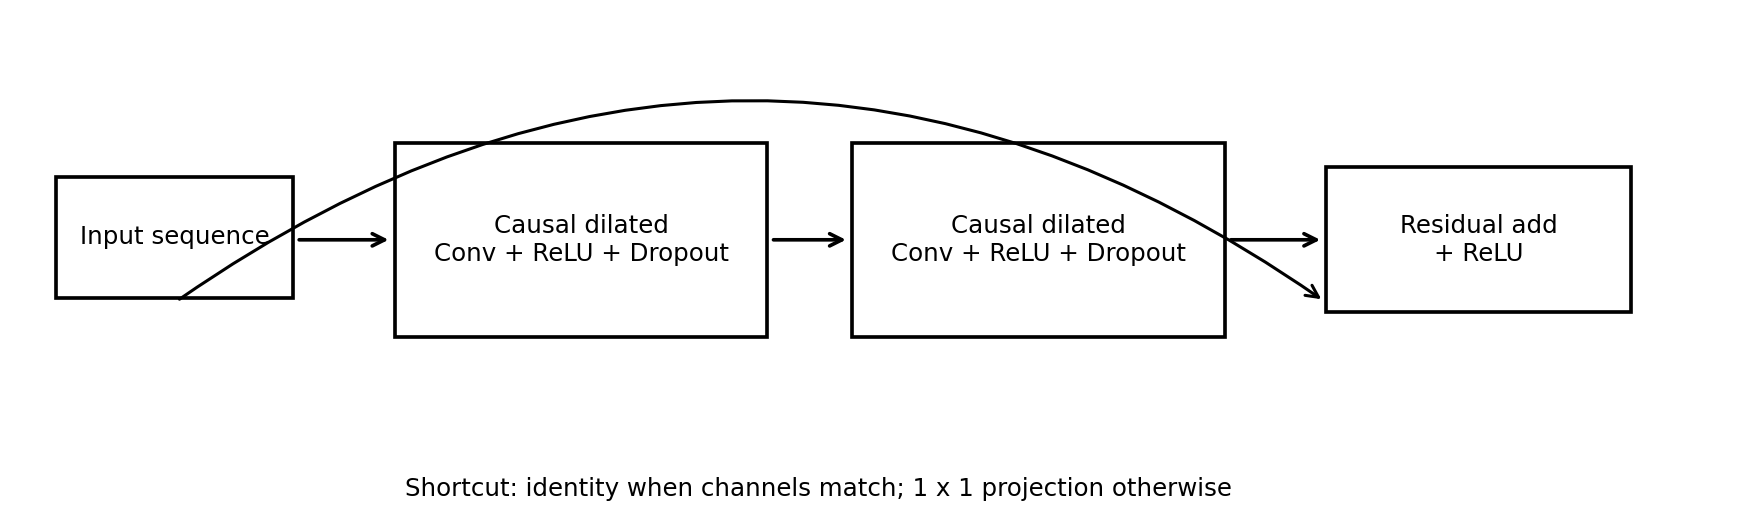
\includegraphics[width=\columnwidth]{figures/tcn_block.png}
\caption{Simplified temporal residual block used in this implementation. The shortcut is an identity mapping or a $1\times1$ projection when channel dimensions differ.}
\label{fig:block}
\end{figure}

The TCN uses weight normalization on convolutional filters. The implementation uses PyTorch's element-wise \texttt{nn.Dropout}; the paper describes spatial dropout, so this regularization detail is not identical to the reference design.

\section{Implementation and Experimental Setup}
\subsection{Code and Validation}
The core architecture is implemented independently in \texttt{tcn.py} through three components: \texttt{CausalConv1d}, \texttt{TemporalBlock}, and \texttt{TemporalConvNet}. Task-specific heads, data generators, recurrent baselines, training loops, and result generation are in the Colab notebook. The notebook imports the project's \texttt{tcn.py} from GitHub and was executed using a Tesla T4 GPU.

Before training, the model was checked for tensor shape, residual compatibility, temporal-length preservation, causality, and receptive-field calculation. For the causality test, inputs after a selected time index were perturbed; outputs up to that index remained unchanged. The test passed. Receptive-field tests also returned 29, 125, and 1,021 for the selected three-, five-, and eight-block configurations.

\subsection{Task Definitions and Configurations}
\textit{Adding Problem:} Each length-100 sample contains two channels. The first contains values sampled from $[0,1]$; the second marks exactly two positions. The target is the sum of the two marked values. Test MSE is reported. The data split contains 4,096 training, 1,024 validation, and 2,048 test samples. Models train for 20 epochs with batch size 128 and Adam learning rate 0.002. The TCN uses five blocks with 16 channels, kernel size three, and dropout 0.1; LSTM and GRU use 48 hidden units.

\textit{Copy Memory:} Each input has length $G+20$, where $G$ is the memory gap. The first ten input positions contain digits from 1 to 8, intermediate positions are zero, and the final eleven input positions contain delimiter token 9. The target is zero except for the final ten positions, which repeat the initial digits. This token layout follows the task definition in the paper \cite{bai2018}. The gap-100 run uses 4,096 / 1,024 / 2,048 training/validation/test examples and 20 epochs. Its full-sequence cross-entropy is unweighted (the final-ten-position weight is 1.0). We report accuracy only on the final ten recall positions because accuracy over all positions would be dominated by zero targets. The gap-20 diagnostic uses 2,048 / 512 / 1,024 examples and 30 epochs; its loss is computed only over the final ten positions. It therefore changes both gap length and loss scope and is not a controlled gap-only comparison.

\textit{Sequential MNIST:} Each $28\times28$ image is flattened in row-major order into 784 pixel values. The model predicts one of ten digit classes from the final sequence representation. The experiment uses 12,000 training images, 2,000 validation images from the MNIST training split, and 5,000 test images for eight epochs, with batch size 128 and Adam learning rate 0.001. The TCN uses eight blocks of 16 channels and kernel size three (12,282 parameters); LSTM and GRU use hidden size 64 (17,802 and 13,514 parameters).

\begin{table}[t]
\caption{Main Experimental Settings}
\label{tab:settings}
\centering
\scriptsize
\begin{tabular}{p{0.20\columnwidth}p{0.37\columnwidth}p{0.34\columnwidth}}
\toprule
Task & Data and training & Model configuration\\
\midrule
Adding & Length 100; 4,096/1,024/2,048; 20 epochs & TCN: 5 blocks, 16 channels, $k=3$; LSTM/GRU: 48 hidden units\\
Copy, $G=100$ & Length 120; 4,096/1,024/2,048; 20 epochs & TCN: 5 blocks, 16 channels, $k=3$; LSTM/GRU: 64 hidden units\\
Copy, $G=20$ & Length 40; 2,048/512/1,024; 30 epochs & Same architecture families as long-gap run\\
Seq. MNIST & 784 pixels; 12,000/2,000/5,000; 8 epochs & TCN: 8 blocks, 16 channels, $k=3$; LSTM/GRU: 64 hidden units\\
Ablation & Adding split; 20 epochs & Five 16-channel blocks; dilation schedule changed\\
\bottomrule
\end{tabular}
\end{table}

\subsection{Seeds}
Adding Problem uses data seeds 101, 202, and 303 and model seeds 1000--1002. Copy Memory gap 100 uses data seeds 101, 202, and 303 and model seeds 3000--3002. Gap 20 uses data seeds 401, 402, and 403 and model seeds 5000--5002. Sequential MNIST uses split seed 12345 (test split seed 12346) and model seeds 6000--6002. The ablation uses the same Adding Problem split and model seeds 7101 and 7102. These are single runs; no repeated-seed averages or confidence intervals were computed.

\section{Results and Discussion}
\subsection{Adding Problem}
Table~\ref{tab:adding} shows the test MSE for each model. TCN and GRU learn the task and perform substantially better than the constant-prediction baseline of 0.171037. The LSTM's MSE is 0.170794, only 0.000243 below the baseline, so it is best interpreted as approximately baseline performance rather than meaningful learning. The paper reports results at sequence length $T=600$ with larger models; our sequence length is 100, so the values are not a like-for-like reproduction.

\begin{table}[t]
\caption{Adding Problem Test MSE}
\label{tab:adding}
\centering
\scriptsize
\begin{tabular}{lrrr}
\toprule
Model & Our MSE ($T=100$) & Paper loss ($T=600$) & Baseline MSE\\
\midrule
TCN & \textbf{0.013983} & $5.8\times10^{-5}$ & 0.171037\\
LSTM & 0.170794 & 0.164 & 0.171037\\
GRU & 0.012469 & $5.3\times10^{-5}$ & 0.171037\\
\bottomrule
\end{tabular}
\end{table}

\begin{figure}[t]
\centering
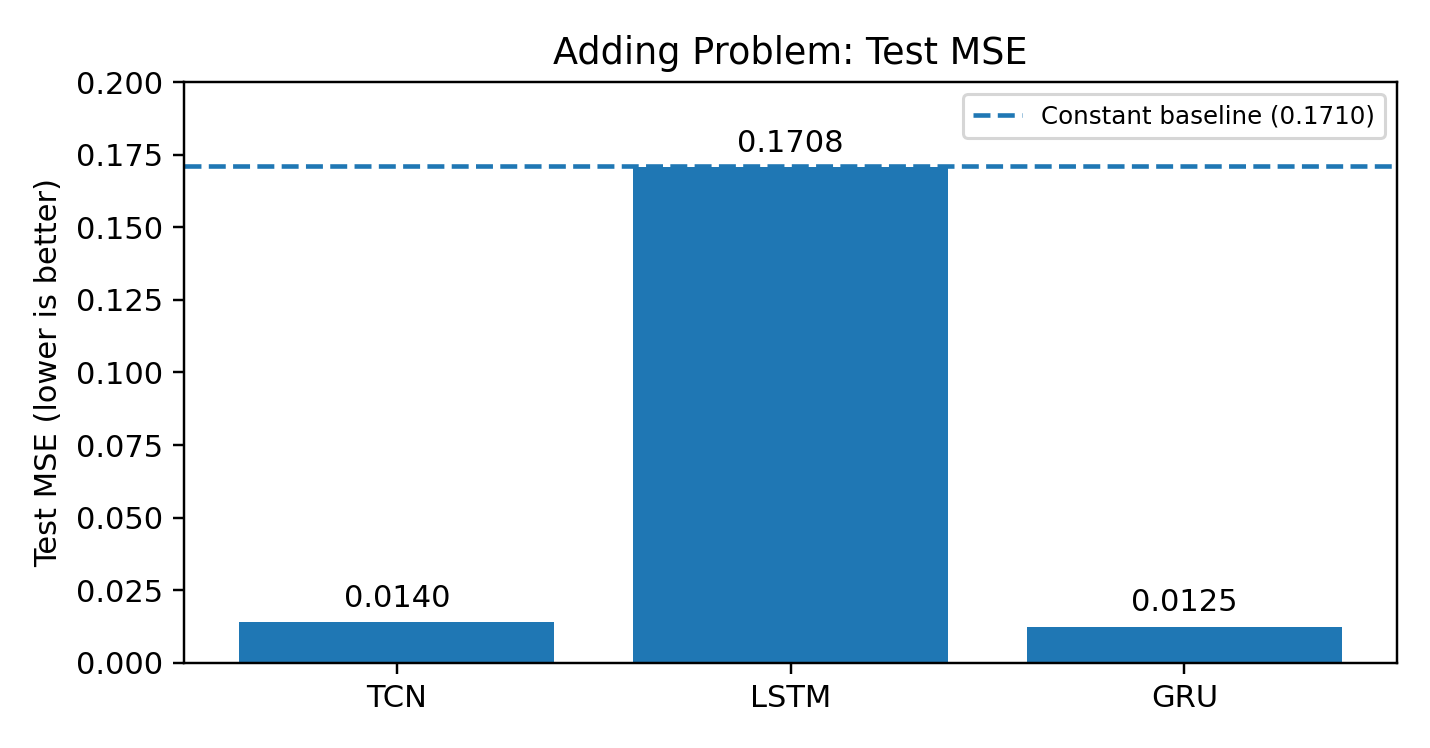
\includegraphics[width=\columnwidth]{figures/adding_problem.png}
\caption{Adding Problem test MSE and constant-prediction baseline.}
\label{fig:adding}
\end{figure}

\subsection{Copy Memory}
For gap 100, the total input length is 120. The TCN, LSTM, and GRU obtain 12.53\%, 12.22\%, and 12.34\% recall accuracy, respectively (Table~\ref{tab:copy}). Because the target digits are sampled uniformly from 1 to 8, uniform guessing among the eight valid digits has expected per-digit accuracy of 12.5\%. The results are therefore near chance and do not demonstrate reliable long-gap recall. The all-zero predictor obtains 0\% on the final ten target positions because those target digits are never zero. The paper reports Copy Memory loss at $T=1000$ (TCN $3.5\times10^{-5}$, LSTM 0.0204, GRU 0.0197); our gap is shorter and we report recall accuracy, so the numerical values are not directly comparable.

The gap-20 diagnostic obtains 100\% digit and exact-sequence accuracy with the TCN. However, this experiment also changes the loss from full-sequence cross-entropy to recall-only cross-entropy. The LSTM obtains 12.42\% digit accuracy and the GRU 30.56\%; neither produces a fully correct ten-digit sequence in the test set. The short-gap result is a useful diagnostic of the implementation, not evidence that gap length alone explains the change. Figure~\ref{fig:copy} presents both runs.

\begin{table}[t]
\caption{Copy Memory Recall Results}
\label{tab:copy}
\centering
\scriptsize
\begin{tabular}{lrrr}
\toprule
Model & Gap 100 acc. & Gap 20 acc. & Gap 20 exact\\
\midrule
TCN & 12.53\% & \textbf{100.00\%} & \textbf{100.00\%}\\
LSTM & 12.22\% & 12.42\% & 0.00\%\\
GRU & 12.34\% & 30.56\% & 0.00\%\\
\bottomrule
\end{tabular}
\end{table}

\begin{figure}[t]
\centering
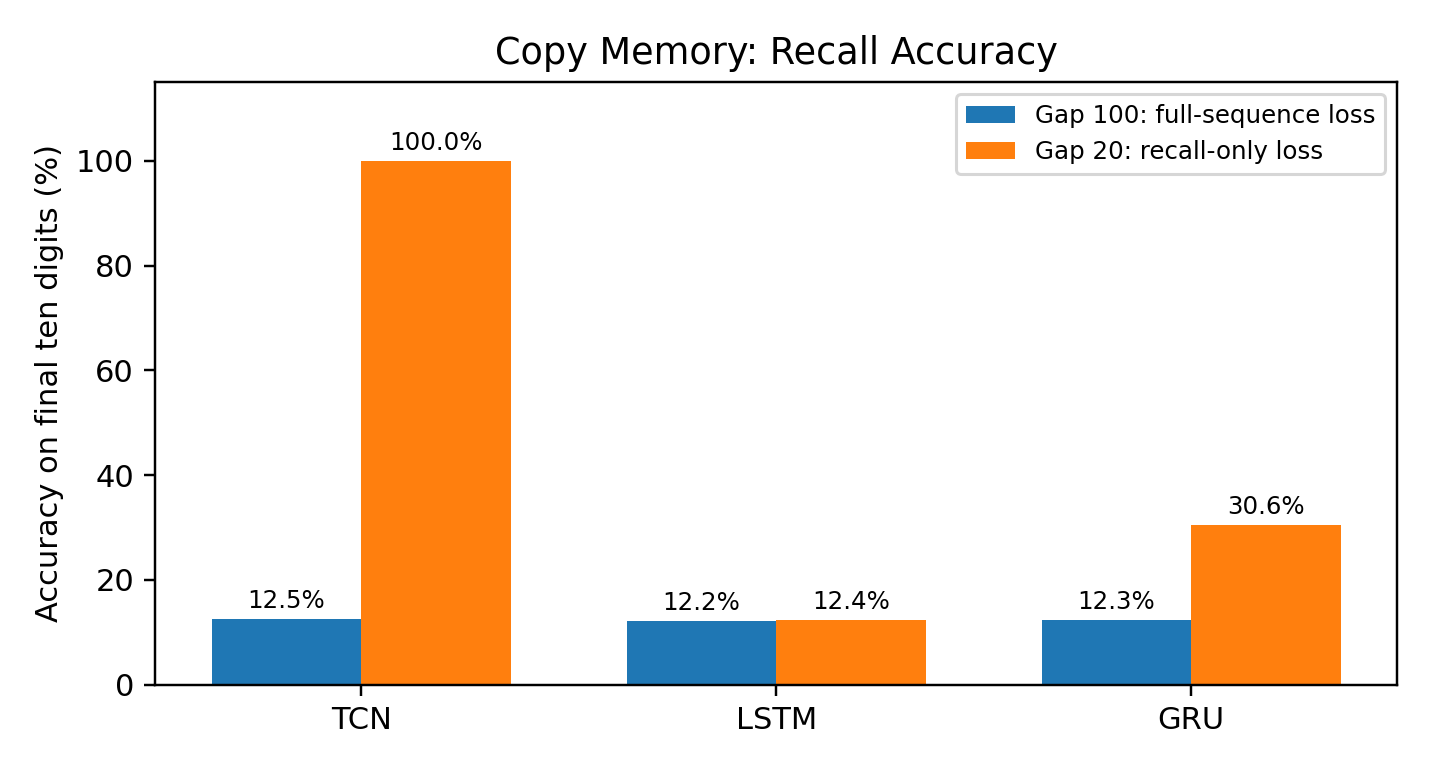
\includegraphics[width=\columnwidth]{figures/copy_memory.png}
\caption{Copy Memory recall accuracy on the final ten digits. The gap-20 run uses recall-only loss and is a diagnostic.}
\label{fig:copy}
\end{figure}

\subsection{Sequential MNIST}
The TCN reaches 91.62\% test accuracy, compared with 11.08\% for the LSTM and 42.32\% for the GRU (Table~\ref{tab:mnist}). The paper reports 99.0\%, 87.2\%, and 96.2\% for TCN, LSTM, and GRU, respectively. Our run uses fewer training examples, fewer epochs, and smaller models. The LSTM training loss remains close to $-\log(0.1)\approx2.3026$, the cross-entropy of uniform predictions over ten classes, indicating that it did not learn adequately. The GRU learned partially but did not converge to a strong result within eight epochs. Recurrent baselines were not extensively tuned, so these outcomes should not be interpreted as evidence that recurrent models are inherently inferior.

\begin{table}[t]
\caption{Sequential MNIST Test Accuracy}
\label{tab:mnist}
\centering
\begin{tabular}{lrrr}
\toprule
Model & Parameters & Our accuracy & Paper accuracy\\
\midrule
TCN & 12,282 & \textbf{91.62\%} & 99.0\%\\
LSTM & 17,802 & 11.08\% & 87.2\%\\
GRU & 13,514 & 42.32\% & 96.2\%\\
\bottomrule
\end{tabular}
\end{table}

\begin{figure}[t]
\centering
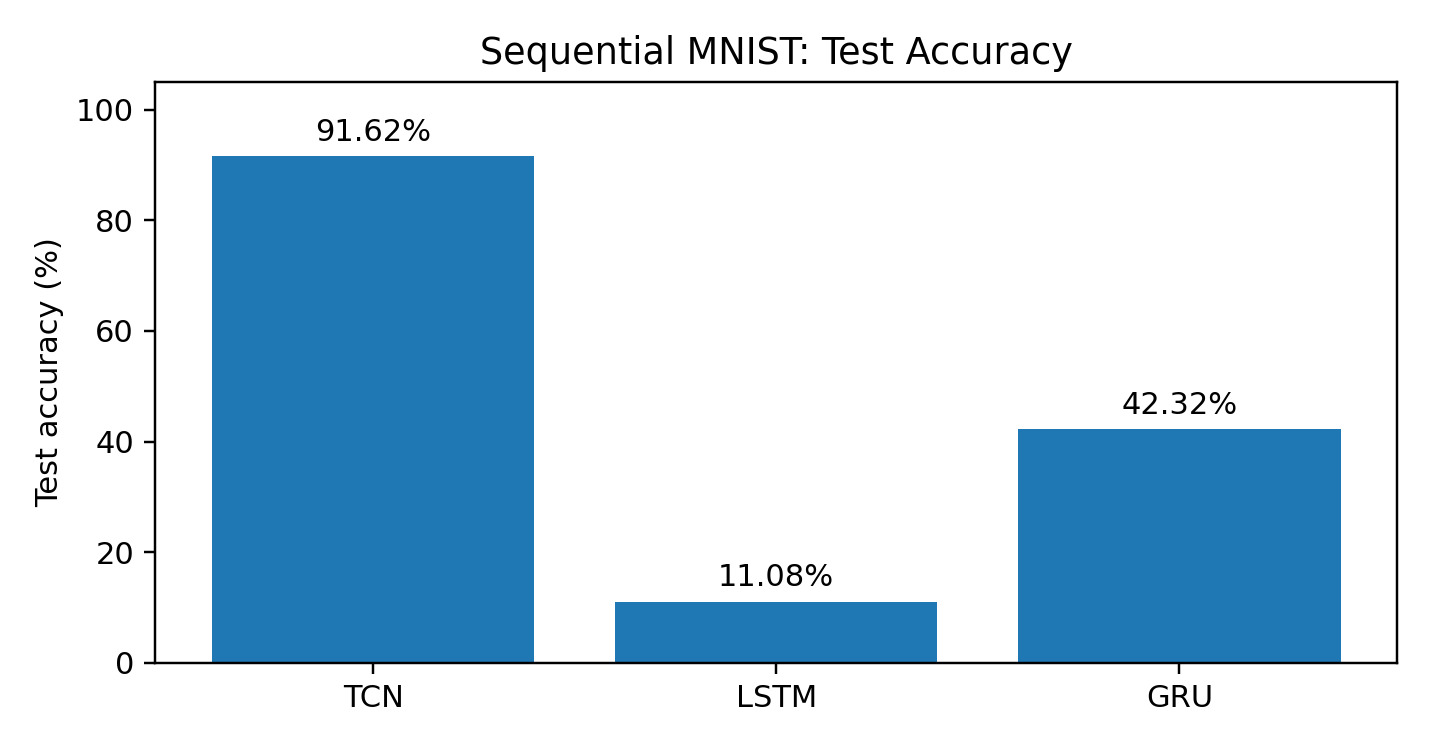
\includegraphics[width=\columnwidth]{figures/sequential_mnist.png}
\caption{Sequential MNIST test accuracy in the reduced-scale run.}
\label{fig:mnist}
\end{figure}

\subsection{Dilation Ablation}
The ablation changes the dilation schedule while keeping the Adding Problem data split, five-block depth, 16 channels, kernel size, dropout, batch size, and epoch budget fixed. Both models have 7,393 parameters. The dilated TCN uses dilation factors 1, 2, 4, 8, and 16 and has receptive field 125. The no-dilation model uses dilation one in every block and has receptive field 21. Their test MSEs are 0.020733 and 0.152704, respectively; the constant baseline is 0.171037. This single-run result supports the usefulness of dilation for the tested sequence length and configuration, but it does not establish a general statistical conclusion.

\begin{table}[t]
\caption{Dilation Ablation on the Adding Problem}
\label{tab:ablation}
\centering
\begin{tabular}{lrrr}
\toprule
Configuration & RF & Parameters & Test MSE\\
\midrule
Dilated TCN & 125 & 7,393 & \textbf{0.020733}\\
No dilation & 21 & 7,393 & 0.152704\\
Constant baseline & -- & -- & 0.171037\\
\bottomrule
\end{tabular}
\end{table}

\begin{figure}[t]
\centering
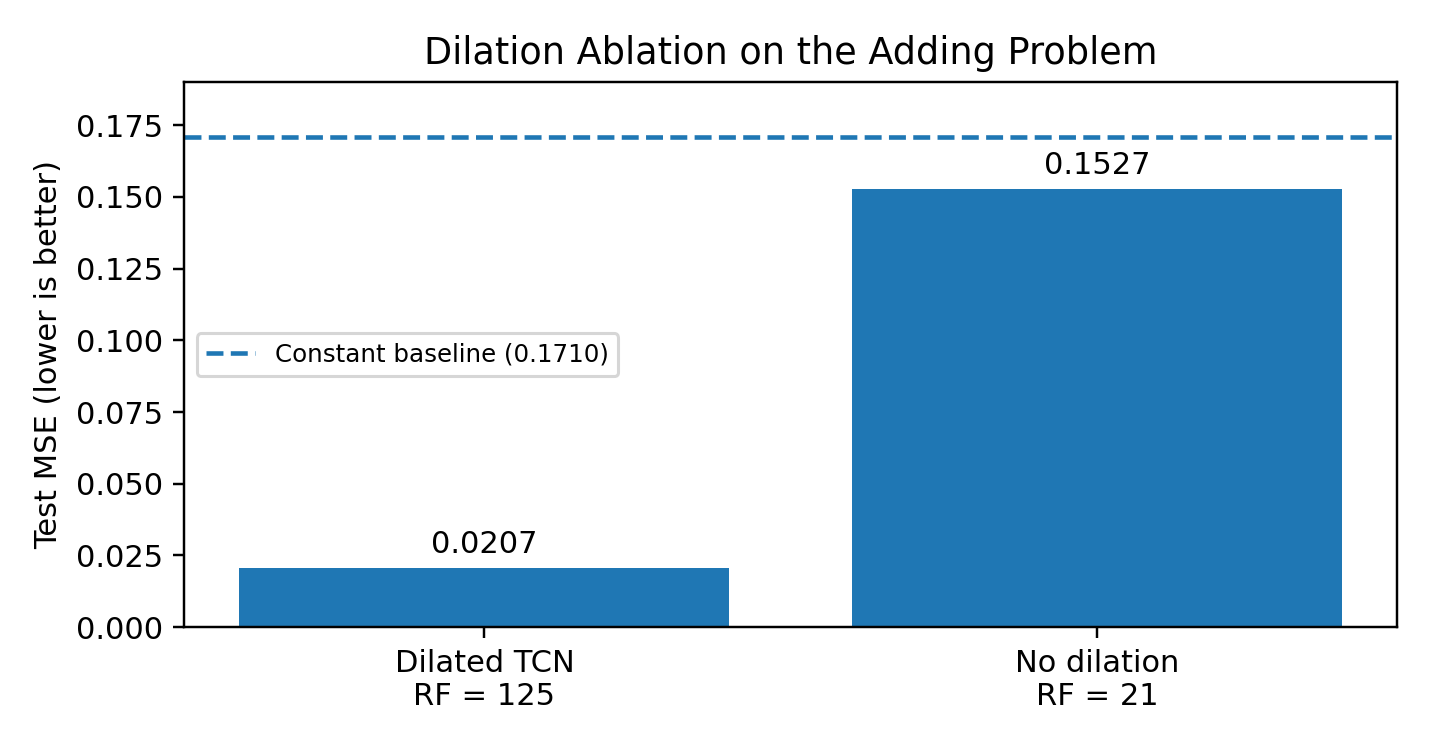
\includegraphics[width=\columnwidth]{figures/dilation_ablation.png}
\caption{Dilation ablation with parameter count held constant.}
\label{fig:ablation}
\end{figure}

\section{Limitations and Conclusion}
The implementation passes the core checks: causality, residual compatibility, sequence-length preservation, and receptive-field calculation. The Adding Problem and Sequential MNIST results favor the TCN in this reduced setup, and the ablation shows lower error with dilation. However, long-gap Copy Memory remains unsolved even though the TCN receptive field spans the input. The short-gap diagnostic changes both gap and loss scope. Recurrent Sequential MNIST baselines are weak and were not extensively tuned. All values are single-run results without repeated-seed statistics.

A stronger follow-up would tune recurrent baselines using validation data, repeat experiments across seeds, and test longer Copy Memory gaps. The current work should be understood as a reduced-scale implementation and empirical study, not an exact reproduction or a claim of universal TCN superiority.

\begin{thebibliography}{2}
\bibitem{bai2018}
S. Bai, J. Z. Kolter, and V. Koltun, ``An Empirical Evaluation of Generic Convolutional and Recurrent Networks for Sequence Modeling,'' arXiv:1803.01271, 2018. [Online]. Available: \url{https://arxiv.org/abs/1803.01271}
\bibitem{locuslab}
S. Bai, J. Z. Kolter, and V. Koltun, ``TCN: Temporal Convolutional Networks,'' reference implementation. [Online]. Available: \url{https://github.com/locuslab/TCN}
\end{thebibliography}
\end{document}
